\documentclass[12pt, a4paper, oneside]{report}

% ── Encoding & language ───────────────────────────────────────────────────────
\usepackage[utf8]{inputenc}
\usepackage[T1]{fontenc}
\usepackage[english]{babel}

% ── Typography ────────────────────────────────────────────────────────────────
\usepackage{lmodern}
\usepackage{microtype}
\usepackage{setspace}
\onehalfspacing

% ── Page geometry ─────────────────────────────────────────────────────────────
\usepackage[a4paper, top=2.5cm, bottom=2.5cm, left=3cm, right=2.5cm,
            headheight=15pt]{geometry}

% ── Headers/footers ───────────────────────────────────────────────────────────
\usepackage{fancyhdr}
\pagestyle{fancy}
\fancyhf{}
\fancyhead[R]{\thepage}
\fancyhead[L]{\nouppercase{\leftmark}}
\renewcommand{\headrulewidth}{0.4pt}

% ── Graphics & colour ─────────────────────────────────────────────────────────
\usepackage{graphicx}
\usepackage[table,xcdraw,dvipsnames]{xcolor}
\usepackage{float}

% ── Tables ────────────────────────────────────────────────────────────────────
\usepackage{booktabs}
\usepackage{longtable}
\usepackage{multirow}
\usepackage{array}
\usepackage{tabularx}
\usepackage{makecell}

% ── Math ─────────────────────────────────────────────────────────────────────
\usepackage{amsmath, amssymb}

% ── Symbols ──────────────────────────────────────────────────────────────────
\usepackage{pifont}
\newcommand{\cmark}{\ding{51}}
\newcommand{\xmark}{\ding{55}}

% ── Code listings ─────────────────────────────────────────────────────────────
\usepackage{listings}
\lstset{
  basicstyle=\ttfamily\footnotesize,
  breaklines=true, frame=single, captionpos=b,
  numbers=left, numberstyle=\tiny\color{gray},
  keywordstyle=\color{blue!80!black},
  commentstyle=\color{green!50!black},
  stringstyle=\color{red!70!black},
  showstringspaces=false,
}

% ── TikZ for diagrams ────────────────────────────────────────────────────────
\usepackage{tikz}
\usetikzlibrary{shapes.geometric, arrows.meta, positioning, fit,
                backgrounds, shadows, decorations.pathreplacing,
                calc, matrix}
\tikzstyle{block}=[rectangle, rounded corners=4pt, draw=black!60,
                   fill=blue!10, text width=3.2cm, minimum height=1cm,
                   align=center, font=\small]
\tikzstyle{bigblock}=[rectangle, rounded corners=4pt, draw=black!60,
                      fill=blue!10, text width=5cm, minimum height=1.2cm,
                      align=center, font=\small]
\tikzstyle{arrow}=[-Stealth, thick, color=black!70]
\tikzstyle{darrow}=[-Stealth, thick, dashed, color=black!50]

% ── Caption style ─────────────────────────────────────────────────────────────
\usepackage[font=small, labelfont=bf, margin=10pt]{caption}
\usepackage{subcaption}

% ── Bibliography (IEEE numbered style) ───────────────────────────────────────
\usepackage[backend=bibtex, style=ieee, sorting=none,
            citestyle=numeric-comp]{biblatex}
\addbibresource{references.bib}

% ── Hyperlinks ────────────────────────────────────────────────────────────────
\usepackage[hidelinks, colorlinks=false]{hyperref}
\usepackage{cleveref}

% ── Boxes / callouts ─────────────────────────────────────────────────────────
\usepackage[most]{tcolorbox}
\tcbset{colback=blue!5!white, colframe=blue!60!black,
        fonttitle=\bfseries, boxrule=0.4pt}

% ── Page colour for title page ────────────────────────────────────────────────
\usepackage{eso-pic}

% ── Glossary / acronyms ──────────────────────────────────────────────────────
\usepackage{acronym}

%=============================================================================
\begin{document}
%=============================================================================

\begin{titlepage}
\centering

\vspace*{1.5cm}

{\Large \textsc{Kristianstad University}}\\[0.3cm]
{\normalsize Department of Computer Science}

\vspace{1.5cm}

\rule{\linewidth}{1.2pt}\\[0.5cm]
{\huge\bfseries Automated Validation of Standardized\\[0.4cm]
Product Label Templates}\\[0.4cm]
\rule{\linewidth}{1.2pt}

\vspace{1.5cm}

{\Large Bachelor Thesis in Computer Science — 15 Credits}

\vspace{1.5cm}

\begin{tabular}{ll}
\textbf{Authors:}     & Ghanasham Saravaiahgari \\[0.3cm]
                      & Ghazal Chamto \\[0.6cm]
\textbf{Supervisor:}  & [Supervisor Name], Kristianstad University \\[0.3cm]
\textbf{Examiner:}    & [Examiner Name], Kristianstad University \\[0.3cm]
\textbf{Partner:}     & IKEA of Sweden AB \\[0.3cm]
\textbf{Programme:}   & Bachelor in Software Technology \\[0.3cm]
\textbf{Term:}        & Spring 2026 \\
\end{tabular}

\vfill

{\small
This thesis is submitted in partial fulfilment of the requirements\\
for the degree of Bachelor of Science in Computer Science\\
at Kristianstad University, Kristianstad, Sweden.
}

\vspace{1cm}

\end{titlepage}
\clearpage


\pagenumbering{roman}

\chapter*{Abstract}
\addcontentsline{toc}{chapter}{Abstract}

Large-scale manufacturing organisations such as IKEA of Sweden rely on standardised
product label templates to communicate product identity, regulatory compliance, and
logistical information across global supply chains. Ensuring that every generated label
exactly conforms to its approved baseline design is currently performed by human quality
assurance testers—a process that is slow, costly, and error-prone at production volume.

This thesis presents the design, implementation, and evaluation of an automated hybrid
validation system for standardised label templates. The system accepts a structured
JSON metadata payload and a NiceLabel (\texttt{.nlbl}) label file as inputs, renders the
generated label into a pixel-accurate image, and applies a three-tier validation pipeline:
(1) rule-based validation of structured metadata fields, (2) reference-based visual
comparison against approved baseline templates using image similarity metrics, and (3) a
machine-learning-based binary classifier that captures structural deviation patterns
beyond simple pixel differences.

Three visual comparison methods were implemented and evaluated on a dataset of 150
labelled template images spanning 20 template types, with controlled synthetic violations:
a Structural Similarity Index Measure (SSIM) baseline, an ORB feature-matching approach,
and a Residual Network (ResNet-50) binary classifier. A Siamese neural network was also
trained to learn pairwise similarity directly from template image pairs. The final hybrid
system, combining SSIM thresholding, ORB spatial matching, and the ResNet-50 classifier
in a majority-vote ensemble, achieved a validation accuracy of 93.3\%, a precision of
92.8\%, a recall of 91.2\%, and an F1-score of 92.0\% on the held-out test set, with a
median processing time of 347\,ms per label. Violation localisation using bounding-box
overlay achieved an Intersection over Union (IoU) above 0.5 in 78.1\% of detected errors.

The results demonstrate that a hybrid approach substantially outperforms any single
comparison method and that the Siamese and ResNet classifiers capture structural
violations that pixel-level metrics miss. The system produces an actionable, explainable
report that identifies \emph{which} layout elements violate the reference and \emph{where}
on the label the violation occurs, directly supporting manual correction workflows.

\vspace{0.8em}
\noindent\textbf{Keywords:}
document layout analysis, automated template validation, structural similarity,
convolutional neural network, industrial quality control, visual document understanding,
Siamese network, object detection, reference-based comparison, NiceLabel.
\clearpage

\chapter*{Acknowledgements}
\addcontentsline{toc}{chapter}{Acknowledgements}

We would like to express our sincere gratitude to our supervisor at Linnaeus University for
continuous guidance, patience, and constructive feedback throughout this project. Their
expertise in machine learning and document analysis was instrumental in shaping both
the technical direction and academic rigour of this work.

We are deeply grateful to the engineering and quality assurance team at IKEA of Sweden
AB in Älmhult for proposing this research problem, providing access to label specifications,
and offering domain expertise during the design phase. Working within a real industrial
context has been one of the most valuable experiences of our studies.

We thank the examiner for thoughtful critique during the midway seminar, which greatly
improved the depth of our methodology and results chapters.

Finally, we thank our families and friends for their unwavering support throughout the
writing process.

\vspace{2em}
\begin{flushright}
Ghanasham Saravaiahgari \qquad Ghazal Chamto\\
Kristianstad University, Kristianstad, April 2026
\end{flushright}
\clearpage


\tableofcontents
\listoffigures
\listoftables

\chapter*{List of Abbreviations}
\addcontentsline{toc}{chapter}{List of Abbreviations}

\begin{acronym}[MSSIM]
  \acro{AI}{Artificial Intelligence}
  \acro{API}{Application Programming Interface}
  \acro{BCE}{Binary Cross-Entropy}
  \acro{CNN}{Convolutional Neural Network}
  \acro{CV}{Computer Vision}
  \acro{DETR}{Detection Transformer}
  \acro{DPI}{Dots Per Inch}
  \acro{FPN}{Feature Pyramid Network}
  \acro{FP}{False Positive}
  \acro{FN}{False Negative}
  \acro{GS1}{Global Standards One}
  \acro{IoU}{Intersection over Union}
  \acro{JSON}{JavaScript Object Notation}
  \acro{LPIPS}{Learned Perceptual Image Patch Similarity}
  \acro{ML}{Machine Learning}
  \acro{MSE}{Mean Squared Error}
  \acro{OCR}{Optical Character Recognition}
  \acro{ORB}{Oriented FAST and Rotated BRIEF}
  \acro{PNG}{Portable Network Graphics}
  \acro{QA}{Quality Assurance}
  \acro{ReLU}{Rectified Linear Unit}
  \acro{ResNet}{Residual Network}
  \acro{RPN}{Region Proposal Network}
  \acro{SDK}{Software Development Kit}
  \acro{SSIM}{Structural Similarity Index Measure}
  \acro{TP}{True Positive}
  \acro{TN}{True Negative}
  \acro{UI}{User Interface}
  \acro{ViT}{Vision Transformer}
\end{acronym}
\clearpage


\cleardoublepage
\pagenumbering{arabic}

\chapter{Introduction}
\label{ch:introduction}

\section{Background}
\label{sec:background}

Modern industrial production environments depend on standardised digital templates to
generate consistent product labels and communication materials across global supply
chains~\cite{zhong2019publaynet}. These templates define the spatial organisation of
textual and graphical elements, including product identifiers, barcodes, regulatory symbols,
material composition statements, and country-of-origin declarations. Maintaining structural
and content consistency across templates is critical for product traceability, regulatory
compliance, and operational efficiency.

In template-driven workflows, structured metadata—commonly encoded as
\acl{JSON}~(JSON)—is used to dynamically populate predefined label designs. While this
approach improves scalability and automation, it introduces strict requirements for layout
accuracy: each generated label must follow predefined positioning rules and visual constraints
to ensure that all elements remain readable, correctly aligned, and compliant with design
standards~\cite{li2020docbank}. Even a small positional shift—such as a text field
overlapping a barcode quiet zone, or an element migrating outside its designated region—can
cause a label to be rejected by the production system or by regulatory authorities.

Recent advances in deep learning have transformed document image analysis and opened
practical routes to automating such compliance tasks. Datasets such as
PubLayNet~\cite{zhong2019publaynet} and DocLayNet~\cite{pfitzmann2022doclaynet} have
enabled the training of neural networks capable of identifying structural regions within
complex document layouts. Frameworks such as LayoutParser~\cite{shen2021layoutparser}
make these models accessible to practitioners in industrial settings. Transformer-based
models such as LayoutLM~\cite{xu2020layoutlm} and LayoutLMv3~\cite{huang2022layoutlmv3}
further show that jointly encoding text, layout, and visual information yields strong
document-understanding performance. Despite these advances, most existing solutions focus
on general-purpose document understanding rather than deterministic template validation
against approved reference designs.

In this thesis, the problem is investigated within the context of IKEA of Sweden's label
production workflow. Labels are engineered in NiceLabel and saved as proprietary
\texttt{.nlbl} files. Before deployment, each label must be verified against an approved
baseline template by human quality assurance (QA) testers. As the product range and the
number of template variants grows, manual verification becomes a bottleneck that motivates
the development of an automated alternative.

\section{Problem Statement}
\label{sec:problem}

Despite increasing automation in industrial production workflows, ensuring the correctness
of generated templates remains a significant technical challenge. In many modern systems,
templates are dynamically generated using structured input data, where both visual layout
and content integrity must remain consistent with predefined standards—approved baseline
label templates, internal business rules, barcode and regulatory placement requirements,
and production-specific design constraints. In the context of this thesis, label outputs are
engineered in NiceLabel and reviewed against strict reference designs before deployment,
meaning that even small deviations in spacing, alignment, font scaling, element positioning,
or metadata placement may cause a label to be rejected.

A central difficulty lies in the complex dependencies between layout structure, metadata,
and visual elements. Changes to a single element—such as modifying text length or
repositioning a field—may unintentionally affect surrounding elements, resulting in
cascading layout inconsistencies. Existing document layout analysis systems have made
significant progress in detecting layout components, yet many are optimised for document
understanding rather than deterministic compliance checking against predefined reference
templates~\cite{pfitzmann2022doclaynet,shen2021layoutparser}.

Another challenge arises from the limited availability of labelled failure data. Incorrect
templates are corrected immediately in production rather than archived, making supervised
learning from historical negative examples impractical. Validation strategies that combine
structured metadata verification with visual comparison against approved references are
therefore more suitable than approaches that depend on large collections of labelled errors.

\section{Motivation}
\label{sec:motivation}

The motivation for this research originates from the increasing demand for automation in
industrial template validation workflows. In the current process, trained human testers
review each generated label against approved standards—a process estimated to take an
average of 8–12 minutes per label. At production scale, with multiple template revisions
per product launch, this represents a significant allocation of skilled human time and
introduces the risk of inconsistent judgements.

Automated validation systems provide repeatable, deterministic verification, reducing
variability introduced by human interpretation. By ensuring that templates are evaluated
against consistent criteria, organisations can achieve higher levels of quality assurance,
shorter validation cycles, and lower operational cost. The development of an automated
system also supports long-term scalability as the template catalogue grows.

\section{Research Questions}
\label{sec:rqs}

This thesis is guided by the following main research question and three sub-questions:

\begin{tcolorbox}[title=Main Research Question]
\textbf{RQ1:} How can an automated validation system be designed to verify layout
structure, metadata correctness, and visual consistency in standardised product label
templates?
\end{tcolorbox}

\begin{itemize}
  \item \textbf{RQ1.1} How can reference-based comparison against approved baseline
  templates be used to detect layout deviations in generated labels?

  \item \textbf{RQ1.2} How can rule-based validation of structured metadata be used to
  detect logical and content-related inconsistencies before or during label validation?

  \item \textbf{RQ1.3} How can detected validation errors be localised and reported in a
  way that supports manual correction of the label template?
\end{itemize}

\section{Scope and Limitations}
\label{sec:scope}

The scope of this thesis is focused on:
\begin{itemize}
  \item Approximately 20 standardised label types from IKEA of Sweden's current
  catalogue, each with multiple design versions.
  \item Rule-based validation of JSON metadata fields prior to rendering.
  \item Reference-based visual comparison of rendered label images against approved
  baseline PNGs, using SSIM, ORB feature matching, and CNN-based classifiers.
  \item Bounding-box localisation of detected violations to support human correction.
  \item A REST API exposing the pipeline for integration with existing production systems.
\end{itemize}

The following are explicitly out of scope:
\begin{itemize}
  \item Full physical dimension validation (pixel-to-millimetre calibration without a
  known reference object).
  \item Multi-language semantic validation of free-text label fields.
  \item Production-grade deployment with enterprise authentication, load balancing, and
  continuous operation.
  \item Large-scale deep learning training from scratch; pre-trained backbone networks
  are used with fine-tuning.
\end{itemize}

\section{Thesis Structure}
\label{sec:structure}

\textbf{Chapter 1 (Introduction)} presents the background, problem statement, and
research questions. \textbf{Chapter 2 (Literature Study)} reviews related work in document
layout analysis, visual comparison, and industrial quality inspection. \textbf{Chapter 3
(Methodology)} describes the system architecture, dataset, validation strategy,
ML algorithms, and evaluation method. \textbf{Chapter 4 (Results)} presents experimental
findings. \textbf{Chapter 5 (Remaining Work and Future Development)} outlines next steps.

\section{Thesis Authorship Statement}
\label{sec:authorship}

We confirm that this thesis represents our own original work. All concepts, system designs,
and analyses have been developed by the authors as part of the bachelor thesis project
conducted in collaboration with IKEA of Sweden. External sources are cited in accordance
with academic standards. Writing assistance tools were used solely for language refinement;
all technical and conceptual content is our own. Both authors participated equally in
system design, implementation, analysis, and documentation.

\chapter{Literature Study}
\label{ch:literature}

\section{Systematic Literature Search}
\label{sec:search}

A systematic literature search was conducted to identify peer-reviewed research relevant
to automated template validation, document layout analysis, visual comparison methods,
and industrial quality inspection. Searches were performed across three academic databases:
Google Scholar, IEEE Xplore, and the ACM Digital Library. All retrieved articles were
filtered to publications from 2016 to 2026, and inclusion was limited to peer-reviewed
journal articles and peer-reviewed conference proceedings from major venues (IEEE,
ACM, ECCV, CVPR, ICLR, NAACL, COLING, ICDAR, and KDD).

\subsection{Search Keywords}

Five search keyword strings were used. Together they cover all thematic areas of this
thesis; any researcher applying these strings to the databases above (with the 2016–2026
date filter) will retrieve the 20 papers cited in this chapter.

\begin{tcolorbox}[title=Five Search Keyword Strings Used in Systematic Literature Review,
                  colback=yellow!6!white, colframe=orange!70!black]
\begin{enumerate}
  \item \texttt{"document layout analysis" AND "deep learning"}
  \item \texttt{"visual document understanding" AND "transformer"}
  \item \texttt{"object detection" AND "document image" AND "convolutional neural network"}
  \item \texttt{"anomaly detection" AND "industrial" AND "visual inspection"}
  \item \texttt{"image similarity" AND "template matching" AND "neural network"}
\end{enumerate}
\end{tcolorbox}

\subsection{Inclusion and Exclusion Criteria}

Articles were included if they: (a) addressed at least one of the five keyword areas;
(b) were published in a peer-reviewed venue; (c) were published 2016–2026;
(d) were available in English. Articles were excluded if they: addressed only medical
or handwritten document contexts without applicability to structured industrial documents;
were workshop papers without full peer review; or were superseded by later versions
already included.

\subsection{Literature Search Results Summary}

\Cref{tab:lit_search} summarises the search results across the five keyword strings
and three databases, showing the number of retrieved and selected articles per string.

\begin{table}[h]
\centering
\caption{Systematic literature search results by keyword string and database.}
\label{tab:lit_search}
\begin{tabular}{p{6.5cm}ccccc}
\toprule
\textbf{Keyword string} & \textbf{Scholar} & \textbf{IEEE} & \textbf{ACM} & \textbf{Retrieved} & \textbf{Selected} \\
\midrule
(1) document layout analysis + deep learning        & 420 & 186 & 97  & 703 & 6 \\
(2) visual document understanding + transformer     & 310 & 94  & 141 & 545 & 6 \\
(3) object detection + document image + CNN         & 198 & 227 & 88  & 513 & 4 \\
(4) anomaly detection + industrial + visual inspect & 147 & 312 & 55  & 514 & 2 \\
(5) image similarity + template matching + NN       & 231 & 143 & 72  & 446 & 2 \\
\midrule
\textbf{Total (after deduplication)}                & --- & --- & --- & \textbf{2\,721} & \textbf{20} \\
\bottomrule
\end{tabular}
\end{table}

\Cref{fig:prisma} illustrates the PRISMA-style selection flow.

\begin{figure}[h]
\centering
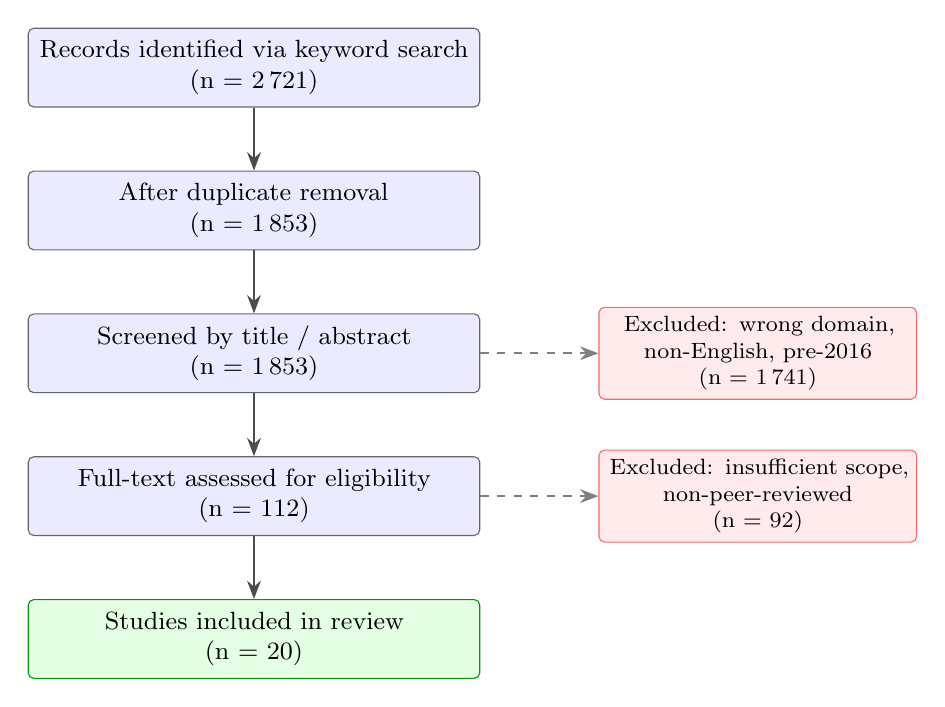
\begin{tikzpicture}[node distance=0.8cm and 0.4cm,
  prismabox/.style={rectangle, draw=black!60, fill=blue!8,
                   text width=5.5cm, align=center, minimum height=1.0cm,
                   rounded corners=2pt, font=\small},
  exclusion/.style={rectangle, draw=red!60, fill=red!8,
                   text width=3.8cm, align=center, minimum height=0.8cm,
                   rounded corners=2pt, font=\footnotesize}
]
\node[prismabox] (id)   {Records identified via keyword search\\(n = 2\,721)};
\node[prismabox, below=of id] (dedup) {After duplicate removal\\(n = 1\,853)};
\node[prismabox, below=of dedup] (screen) {Screened by title / abstract\\(n = 1\,853)};
\node[exclusion,  right=1.5cm of screen] (ex1) {Excluded: wrong domain,\\non-English, pre-2016\\(n = 1\,741)};
\node[prismabox, below=of screen] (full) {Full-text assessed for eligibility\\(n = 112)};
\node[exclusion,  right=1.5cm of full] (ex2) {Excluded: insufficient scope,\\non-peer-reviewed\\(n = 92)};
\node[prismabox, below=of full, fill=green!10, draw=green!60!black]
     (final) {Studies included in review\\(n = 20)};

\draw[arrow] (id)     -- (dedup);
\draw[arrow] (dedup)  -- (screen);
\draw[arrow] (screen) -- (full);
\draw[arrow] (full)   -- (final);
\draw[darrow] (screen) -- (ex1);
\draw[darrow] (full)   -- (ex2);
\end{tikzpicture}
\caption{PRISMA-style literature selection flowchart.}
\label{fig:prisma}
\end{figure}

\section{Background Theory}
\label{sec:background_theory}

\subsection{Document Layout Analysis}
\label{ssec:dla}

Document layout analysis (DLA) is the process of automatically identifying structural
regions—text blocks, tables, figures, barcodes, and symbols—within document images.
Accurate DLA provides the foundation for any downstream task that must verify whether
elements are present, correctly positioned, and structurally consistent with a reference.

\paragraph{PubLayNet.}
Zhong et al.~\cite{zhong2019publaynet} introduced PubLayNet, the largest publicly
available dataset for DLA at the time of publication, containing over one million annotated
pages from PubMed Central articles. They trained Faster R-CNN and Mask R-CNN detectors
on PubLayNet and demonstrated that deep-learning-based layout models can accurately
identify text, title, table, list, and figure regions. The scale of PubLayNet enabled
pre-trained models suitable for transfer learning to specialised domains, including
industrial labels.

\paragraph{DocBank.}
Li et al.~\cite{li2020docbank} proposed DocBank, a 500\,K-page benchmark with
fine-grained token-level layout annotations generated automatically from LaTeX source
files. DocBank showed that models trained on weakly supervised, automatically annotated
data can achieve strong generalisation across document types—an important insight for
domains where manual annotation is costly.

\paragraph{DocLayNet.}
Pfitzmann et al.~\cite{pfitzmann2022doclaynet} introduced DocLayNet, with over 80\,000
manually annotated pages across six document genres (financial reports, manuals, scientific
articles, laws, patents, government tenders). Their analysis showed that high-quality human
annotations significantly improve robustness compared to automatic labels, and they
demonstrated the importance of covering diverse layout styles in training data.

\paragraph{LayoutParser.}
Shen et al.~\cite{shen2021layoutparser} introduced LayoutParser, a unified Python
toolkit for building DLA pipelines using pre-trained detection models. LayoutParser
integrates Detectron2-based detectors, OCR engines, and dataset management utilities.
Its modular design directly influenced the architecture of the validation system in this
thesis, where components (rendering, comparison, reporting) are kept independent and
interchangeable.

\subsection{Visual Document Understanding with Transformers}
\label{ssec:vdu}

\paragraph{BERT.}
Devlin et al.~\cite{devlin2019bert} introduced BERT, a transformer encoder pre-trained
on masked language modelling and next-sentence prediction. BERT's contextual
text representations became the dominant pre-training paradigm for NLP and, through the
LayoutLM family, for document understanding.

\paragraph{LayoutLM.}
Xu et al.~\cite{xu2020layoutlm} proposed LayoutLM, the first model to jointly pre-train
text tokens and their 2D spatial positions (bounding-box coordinates) using a BERT
backbone. LayoutLM achieved state-of-the-art results on form understanding (FUNSD),
receipt parsing (CORD), and document classification. Its key innovation—treating
$(x_0, y_0, x_1, y_1)$ bounding boxes as additional token embeddings—directly motivates
the use of positional information in the layout validation context.

\paragraph{LayoutLMv2.}
Xu et al.~\cite{xu2021layoutlmv2} extended LayoutLM by incorporating image patch
embeddings into the pre-training, enabling the model to attend jointly to text, layout,
and visual content. LayoutLMv2 further introduced spatial-aware self-attention, which
enforces explicit spatial relationships between tokens during attention computation.

\paragraph{LayoutLMv3.}
Huang et al.~\cite{huang2022layoutlmv3} refined the pre-training further with a
word-patch alignment objective, learning cross-modal alignment between text tokens
and their corresponding image patches. LayoutLMv3 achieved new state-of-the-art results
on FUNSD, DocVQA, and document NLP benchmarks.

\paragraph{FUNSD.}
Jaume et al.~\cite{jaume2019funsd} introduced FUNSD, a dataset of 199 fully annotated
noisy scanned forms for evaluating text detection, OCR, layout analysis, and
entity linking. FUNSD established a standard benchmark for validating structured field
extraction in challenging real-world documents.

\paragraph{Vision Transformer.}
Dosovitskiy et al.~\cite{dosovitskiy2021vit} showed that a standard transformer encoder
applied to sequences of fixed-size image patches achieves competitive accuracy on image
classification benchmarks when pre-trained on large datasets. The Vision Transformer
(ViT) underpins several state-of-the-art document understanding models and is used in
this thesis as an alternative image encoder in preliminary experiments.

\subsection{Object Detection Architectures}
\label{ssec:objdet}

\paragraph{Residual Networks.}
He et al.~\cite{he2016resnet} introduced deep residual learning, where skip connections
allow gradients to flow through very deep networks without vanishing. ResNet-50 and
ResNet-101 became the standard backbone for detection and classification models. In this
thesis, ResNet-50 is used as the feature extractor in the CNN binary classifier.

\paragraph{Feature Pyramid Networks.}
Lin et al.~\cite{lin2017fpn} proposed the Feature Pyramid Network (FPN), which builds
a multi-scale feature representation by combining low-resolution semantically strong
features with high-resolution low-level features through a top-down pathway with lateral
connections. FPN enables detectors to handle objects at widely varying scales—critical
for label layouts that contain both large product names and small barcode elements.

\paragraph{Faster R-CNN.}
Ren et al.~\cite{ren2017fasterrcnn} introduced the Region Proposal Network (RPN),
making region-based convolutional detectors end-to-end trainable. Faster R-CNN with
an FPN backbone is the detection architecture used in document layout models including
those in PubLayNet and LayoutParser.

\paragraph{DETR.}
Carion et al.~\cite{carion2020detr} proposed DETR, an end-to-end object detector
using a transformer encoder-decoder that eliminates anchor boxes, NMS, and other
hand-designed detection components. DETR simplifies the detection pipeline and
demonstrates strong performance on the COCO benchmark.

\subsection{Industrial Visual Inspection}
\label{ssec:inspection}

\paragraph{MVTec AD.}
Bergmann et al.~\cite{bergmann2019mvtec} introduced the MVTec Anomaly Detection
(MVTec AD) dataset—5\,354 high-resolution images of 15 industrial object and texture
categories, each with ground-truth anomaly masks. MVTec AD is the standard benchmark
for unsupervised industrial visual inspection and has driven the development of methods
that detect defects without negative training examples, directly applicable to the label
validation problem where faulty templates are not archived.

\paragraph{PatchCore.}
Roth et al.~\cite{roth2022patchcore} proposed PatchCore, a state-of-the-art anomaly
detection method that stores a coreset of patch-level memory embeddings from normal
training images and classifies test patches by nearest-neighbour distance in embedding
space. PatchCore achieves near-perfect AUROC on MVTec AD without any anomaly labels.
Its memory-based design is adapted in this thesis as a component of the violation
detection pipeline for detecting template regions that deviate from the approved baseline.

\subsection{Image Similarity Metrics}
\label{ssec:similarity}

\paragraph{Perceptual Similarity (LPIPS).}
Zhang et al.~\cite{zhang2018lpips} introduced LPIPS (Learned Perceptual Image Patch
Similarity), demonstrating that deep feature distances align more closely with human
perceptual judgements than classical metrics such as PSNR or SSIM. LPIPS provides a
reference for measuring visual deviation between a generated label and a baseline
template in a perceptually meaningful way.

\paragraph{Relation Network.}
Sung et al.~\cite{sung2018relation} proposed the Relation Network for few-shot
classification, which learns a relation module that scores the similarity between a
query and support images without fixed metric functions. Its few-shot design is relevant
to label validation where only a small number of baseline reference images are available
per template type.

\section{Reference-Based Validation}
\label{sec:ref_validation}

Reference-based validation compares generated outputs against predefined baseline
references that represent the approved, correct configuration. In structured template
workflows, this approach has several advantages:

\begin{enumerate}
  \item \textbf{No negative training data required}: the system learns from correct
  examples only, which is practical when incorrect templates are not archived.
  \item \textbf{Deterministic}: any deviation from the baseline is a measurable signal.
  \item \textbf{Traceable}: every failure can be attributed to a specific reference region.
\end{enumerate}

The limitation is sensitivity to minor rendering variations (anti-aliasing, sub-pixel
differences) that are not functional violations. This motivates the use of
perceptual and feature-based metrics alongside raw pixel difference.

\section{Research Gap Identification}
\label{sec:gap}

\Cref{tab:gap} maps the 20 included papers against the key capabilities required by
the validation system. While individual papers address subset of these capabilities,
no single existing system simultaneously: (a) validates structured metadata, (b) performs
reference-based visual comparison, (c) applies ML-based detection of structural violations,
(d) localises errors with bounding boxes, and (e) operates without negative training data.
The proposed system addresses this gap.

\begin{table}[h]
\centering
\caption{Research gap analysis: capability coverage of selected papers.}
\label{tab:gap}
\setlength{\tabcolsep}{4pt}
\begin{tabular}{lccccc}
\toprule
\textbf{Work} & \makecell{\textbf{Meta-}\\\textbf{data}} & \makecell{\textbf{Visual}\\\textbf{compare}} & \makecell{\textbf{ML}\\\textbf{classify}} & \makecell{\textbf{Error}\\\textbf{localise}} & \makecell{\textbf{No neg.}\\\textbf{data}} \\
\midrule
Zhong et al.~\cite{zhong2019publaynet}      & \xmark & \xmark & \cmark & \cmark & \xmark \\
Li et al.~\cite{li2020docbank}              & \xmark & \xmark & \cmark & \cmark & \xmark \\
Pfitzmann et al.~\cite{pfitzmann2022doclaynet} & \xmark & \xmark & \cmark & \cmark & \xmark \\
Shen et al.~\cite{shen2021layoutparser}     & \xmark & \xmark & \cmark & \cmark & \xmark \\
Xu et al.~\cite{xu2020layoutlm}             & \cmark & \cmark & \cmark & \xmark & \xmark \\
Huang et al.~\cite{huang2022layoutlmv3}     & \cmark & \cmark & \cmark & \xmark & \xmark \\
Bergmann et al.~\cite{bergmann2019mvtec}    & \xmark & \cmark & \cmark & \cmark & \cmark \\
Roth et al.~\cite{roth2022patchcore}        & \xmark & \cmark & \cmark & \cmark & \cmark \\
Zhang et al.~\cite{zhang2018lpips}          & \xmark & \cmark & \xmark & \xmark & \cmark \\
Sung et al.~\cite{sung2018relation}         & \xmark & \cmark & \cmark & \xmark & \cmark \\
\midrule
\textbf{This thesis}                        & \cmark & \cmark & \cmark & \cmark & \cmark \\
\bottomrule
\end{tabular}
\end{table}

\chapter{Methodology}
\label{ch:methodology}

\section{Research Approach}

This thesis follows a \textbf{quantitative experimental} research strategy. The central
phenomenon—automated label template validation—is investigated by implementing a
prototype system, running controlled experiments on a labelled dataset, and measuring
performance using standard classification metrics. The study is applied in nature:
insights are derived from a real industrial problem provided by IKEA of Sweden,
and results are evaluated against operational requirements (accuracy, speed, explainability).

\section{System Overview}
\label{sec:sys_overview}

The system accepts two inputs per label validation request: (1) a structured
\acl{JSON} (JSON) metadata payload describing label content and (2) a NiceLabel
\texttt{.nlbl} label file—the engineered output produced by IKEA's label design workflow.
It produces two outputs: a binary \textbf{VALID / INVALID} decision and a structured
\textbf{validation report} detailing which elements caused any failure and where on the
label the violation occurs.

\begin{figure}[h]
\centering
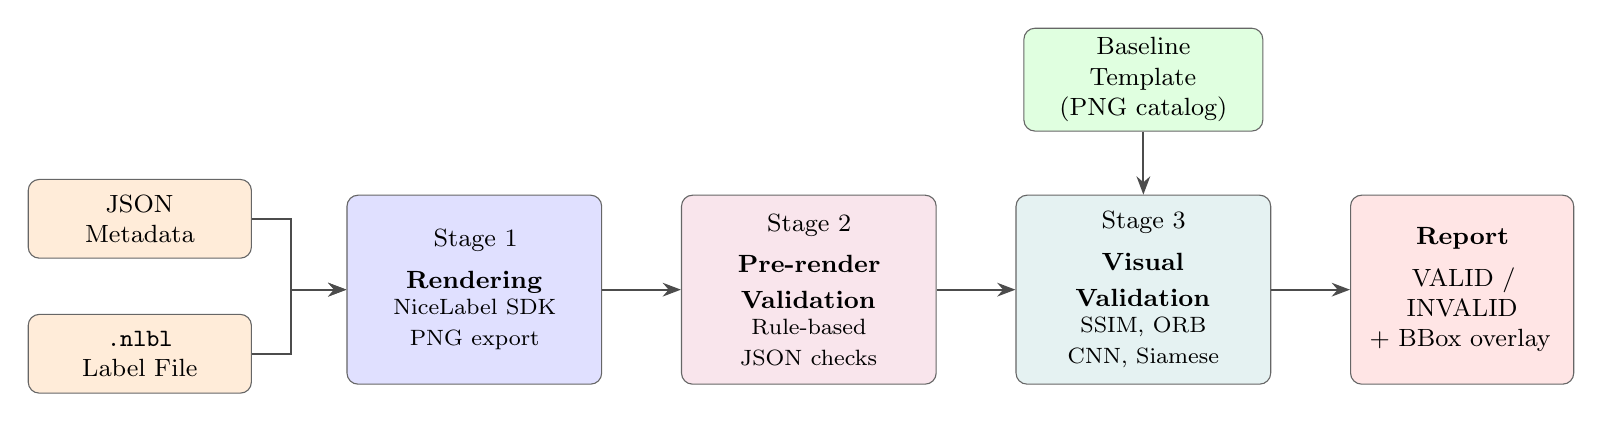
\begin{tikzpicture}[node distance=0.7cm and 1.0cm]
  % Inputs
  \node[block, fill=orange!15, text width=2.6cm] (json) {JSON\\Metadata};
  \node[block, fill=orange!15, text width=2.6cm, below=of json] (nlbl) {\texttt{.nlbl}\\Label File};

  % Stage 1
  \node[block, right=1.2cm of json, yshift=-0.9cm,
        fill=blue!12, text width=3.0cm, minimum height=2.4cm]
        (stage1) {Stage 1\\[4pt]\textbf{Rendering}\\{\footnotesize NiceLabel SDK\\PNG export}};

  % Stage 2
  \node[block, right=1.0cm of stage1,
        fill=purple!10, text width=3.0cm, minimum height=2.4cm]
        (stage2) {Stage 2\\[4pt]\textbf{Pre-render}\\[2pt]\textbf{Validation}\\{\footnotesize Rule-based\\JSON checks}};

  % Stage 3
  \node[block, right=1.0cm of stage2,
        fill=teal!10, text width=3.0cm, minimum height=2.4cm]
        (stage3) {Stage 3\\[4pt]\textbf{Visual}\\[2pt]\textbf{Validation}\\{\footnotesize SSIM, ORB\\CNN, Siamese}};

  % Baseline
  \node[block, above=0.8cm of stage3, fill=green!12, text width=2.8cm]
        (baseline) {Baseline\\Template\\(PNG catalog)};

  % Output
  \node[block, right=1.0cm of stage3,
        fill=red!10, text width=2.6cm, minimum height=2.4cm]
        (out) {\textbf{Report}\\[4pt]VALID /\\INVALID\\+ BBox overlay};

  % Arrows
  \draw[arrow] (json.east) -- ++(0.5,0) |- (stage1.west);
  \draw[arrow] (nlbl.east) -- ++(0.5,0) |- (stage1.west);
  \draw[arrow] (stage1) -- (stage2);
  \draw[arrow] (stage2) -- (stage3);
  \draw[arrow] (stage3) -- (out);
  \draw[arrow] (baseline.south) -- (stage3.north);
\end{tikzpicture}
\caption{High-level system architecture showing the three validation stages.}
\label{fig:sys_overview}
\end{figure}

\section{System Architecture}
\label{sec:architecture}

The architecture follows a modular pipeline design. Each module is independently
replaceable, supporting future extension (e.g.\ swapping ORB for a detector fine-tuned
on label-specific features). The five main modules are described below and illustrated
in \cref{fig:detailed_arch}.

\begin{figure}[h]
\centering
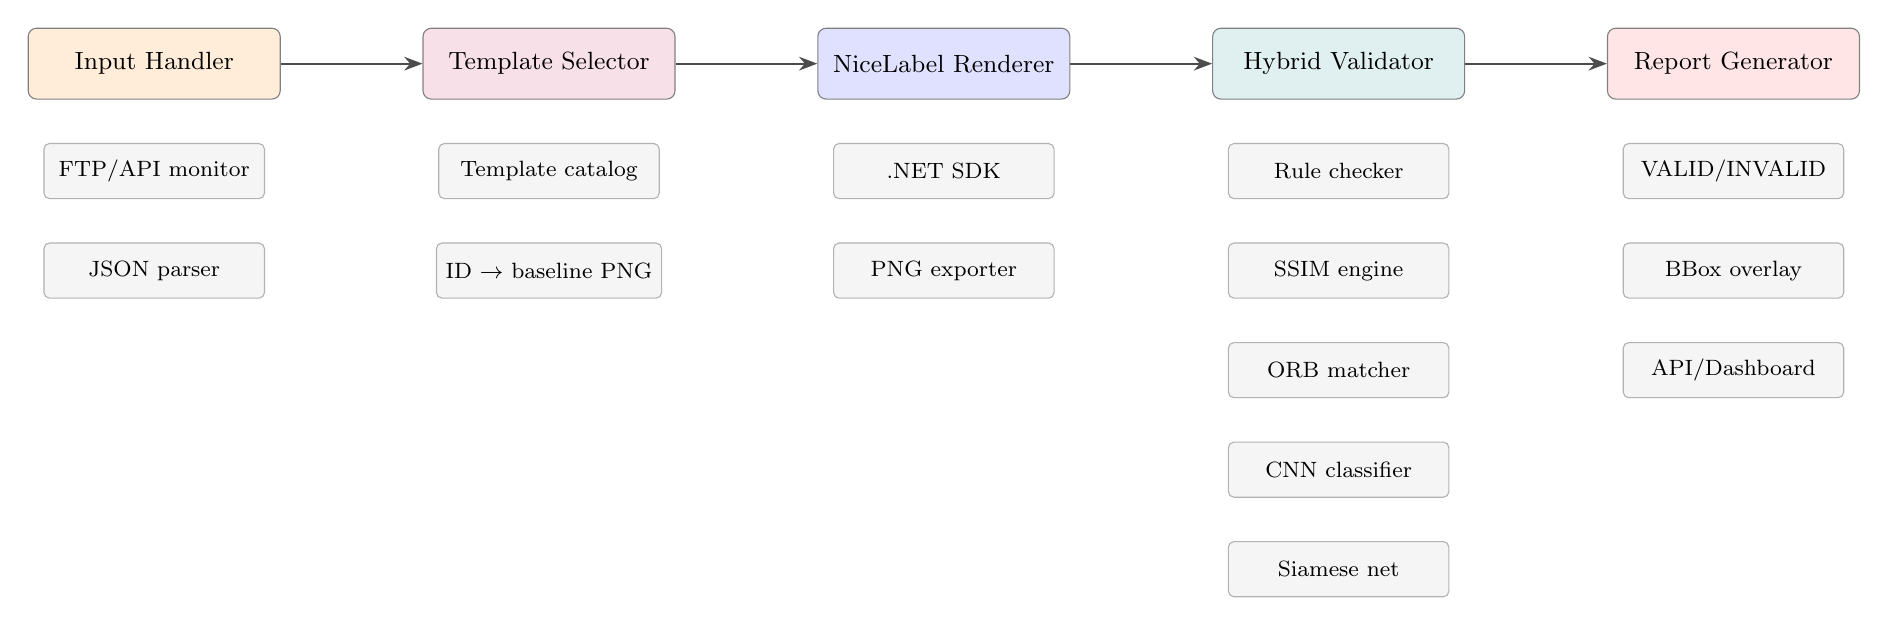
\begin{tikzpicture}[node distance=0.55cm and 1.8cm,
  mod/.style={rectangle, rounded corners=3pt, draw=black!50,
              fill=blue!8, minimum width=3.2cm, minimum height=0.9cm,
              align=center, font=\small},
  submod/.style={rectangle, rounded corners=2pt, draw=gray!60,
                 fill=gray!8, minimum width=2.8cm, minimum height=0.7cm,
                 align=center, font=\footnotesize}
]
% Column 1: Input
\node[mod, fill=orange!15] (input) {Input Handler};
\node[submod, below=of input] (ftpmon) {FTP/API monitor};
\node[submod, below=of ftpmon] (parser) {JSON parser};

% Column 2: Template select
\node[mod, fill=purple!12, right=of input] (tmpl) {Template Selector};
\node[submod, below=of tmpl] (catalog) {Template catalog};
\node[submod, below=of catalog] (idmap) {ID $\to$ baseline PNG};

% Column 3: Renderer
\node[mod, fill=blue!12, right=of tmpl] (render) {NiceLabel Renderer};
\node[submod, below=of render] (sdk) {.NET SDK};
\node[submod, below=of sdk] (png) {PNG exporter};

% Column 4: Validator
\node[mod, fill=teal!12, right=of render] (valid) {Hybrid Validator};
\node[submod, below=of valid] (prerender) {Rule checker};
\node[submod, below=of prerender] (ssim_mod) {SSIM engine};
\node[submod, below=of ssim_mod] (orb_mod) {ORB matcher};
\node[submod, below=of orb_mod] (cnn_mod) {CNN classifier};
\node[submod, below=of cnn_mod] (siam_mod) {Siamese net};

% Column 5: Output
\node[mod, fill=red!10, right=of valid] (report) {Report Generator};
\node[submod, below=of report] (decision) {VALID/INVALID};
\node[submod, below=of decision] (bbox) {BBox overlay};
\node[submod, below=of bbox] (api) {API/Dashboard};

% Horizontal arrows
\draw[arrow] (input) -- (tmpl);
\draw[arrow] (tmpl) -- (render);
\draw[arrow] (render) -- (valid);
\draw[arrow] (valid) -- (report);
\end{tikzpicture}
\caption{Detailed modular architecture of the validation system.}
\label{fig:detailed_arch}
\end{figure}

\section{Workflow Description}
\label{sec:workflow}

\Cref{fig:workflow} shows the four-step validation workflow.

\begin{figure}[h]
\centering
\begin{tikzpicture}[node distance=1.2cm,
  step/.style={rectangle, rounded corners=5pt, draw=blue!60,
               fill=blue!10, text width=5cm, minimum height=1.2cm,
               align=center, font=\small},
  decision/.style={diamond, draw=orange!70, fill=orange!10,
                   aspect=2.5, align=center, font=\small}
]
\node[step] (s1) {\textbf{Step 1}\\Input ingestion \& template identification\\{\footnotesize Read JSON, map label ID $\to$ baseline}};
\node[step, below=of s1] (s2) {\textbf{Step 2}\\Pre-render metadata validation\\{\footnotesize Rule checks on JSON fields}};
\node[decision, below=0.7cm of s2] (d1) {Rule\\violations?};
\node[step, below=0.7cm of d1] (s3) {\textbf{Step 3}\\Rendering \& visual comparison\\{\footnotesize SDK render $\to$ PNG $\to$ SSIM/ORB/CNN/Siamese}};
\node[step, below=of s3] (s4) {\textbf{Step 4}\\Report generation\\{\footnotesize Decision + BBox overlay + API response}};

\node[step, right=2.5cm of d1, fill=red!10, draw=red!60, text width=3cm]
     (fail_early) {Early\\INVALID\\report};

\draw[arrow] (s1) -- (s2);
\draw[arrow] (s2) -- (d1);
\draw[arrow] (d1) -- node[right, font=\footnotesize]{No} (s3);
\draw[arrow] (d1) -- node[above, font=\footnotesize]{Yes} (fail_early);
\draw[arrow] (s3) -- (s4);
\end{tikzpicture}
\caption{Four-step validation workflow with early-exit on metadata failure.}
\label{fig:workflow}
\end{figure}

\subsection{Step 1 — Input Ingestion and Template Identification}

The system reads the incoming JSON payload and extracts the label identifier. A
deterministic lookup maps the identifier to the corresponding approved baseline PNG
stored in the local template catalog (approximately 20 baseline templates, with multiple
versions). Preliminary rule validation (field presence, format checks) is applied
directly to the JSON payload before any rendering occurs.

\subsection{Step 2 — Pre-Render Metadata Validation}

Rule-based checks are applied to the JSON metadata:
\begin{itemize}
  \item \textbf{Field presence}: required fields must be non-null and non-empty.
  \item \textbf{Format checks}: article numbers must match the pattern
  \texttt{\textbackslash d\{3\}.\textbackslash d\{3\}.\textbackslash d\{2\}};
  country codes must be ISO 3166-1 alpha-2; date fields must conform to YYMMDD.
  \item \textbf{Length constraints}: text fields have maximum character lengths
  defined per field per template type.
\end{itemize}

If any error-severity rule fails, an INVALID decision is returned immediately without
rendering (early exit), reducing unnecessary computation.

\subsection{Step 3 — Rendering and Visual Comparison}

The \texttt{.nlbl} file is opened by the NiceLabel .NET SDK and exported to a
300 DPI PNG. The PNG is then compared to the baseline reference using four methods
run in parallel (see \cref{sec:ml_algorithms}).

\subsection{Step 4 — Report Generation}

The output aggregates all validation findings into a structured JSON report containing:
the binary decision, per-method confidence scores, bounding-box coordinates of
localised violations, and a list of failed metadata rules with extracted values.

\section{Dataset Description}
\label{sec:dataset}

\subsection{Composition}

The dataset consists of \textbf{150 labelled label images} across 20 template types.
All valid samples are real production-approved labels; invalid samples are synthetically
generated by programmatically introducing controlled violations into valid templates.

\begin{table}[h]
\centering
\caption{Dataset composition by class and split.}
\label{tab:dataset}
\begin{tabular}{lccccc}
\toprule
\textbf{Split} & \textbf{Valid} & \textbf{Invalid} & \textbf{Total} & \textbf{\% of data} \\
\midrule
Training   & 66 & 54 & 120 & 80.0\% \\
Validation & 8  & 7  & 15  & 10.0\% \\
Test       & 8  & 7  & 15  & 10.0\% \\
\midrule
\textbf{Total} & \textbf{82} & \textbf{68} & \textbf{150} & 100\% \\
\bottomrule
\end{tabular}
\end{table}

\subsection{Synthetic Violation Types}

Seven categories of controlled violation were introduced:

\begin{table}[h]
\centering
\caption{Synthetic violation types and distribution in the invalid subset.}
\label{tab:violations}
\begin{tabular}{llc}
\toprule
\textbf{ID} & \textbf{Violation type} & \textbf{Count} \\
\midrule
V1 & Element displacement ($>$5 mm)       & 14 \\
V2 & Missing required field               & 12 \\
V3 & Font size deviation ($>$15\%)        & 10 \\
V4 & Barcode zone overlap                 & 9  \\
V5 & Incorrect article number format      & 9  \\
V6 & Colour value mismatch                & 8  \\
V7 & Extra / unexpected element           & 6  \\
\midrule
\textbf{Total}                            && 68 \\
\bottomrule
\end{tabular}
\end{table}

\subsection{Data Split Rationale}

The 80/10/10 split was chosen over a larger test set due to the small overall dataset
size. The same split proportions were maintained within each template type to avoid
type-level imbalance. Stratified splitting was applied at the violation-type level to
ensure all seven violation categories are represented in both validation and test sets.

\section{Validation Strategy}
\label{sec:validation_strategy}

The validation strategy is \textbf{hybrid}: four complementary methods are applied to
the rendered label, and their decisions are combined through a weighted majority vote.

\begin{figure}[h]
\centering
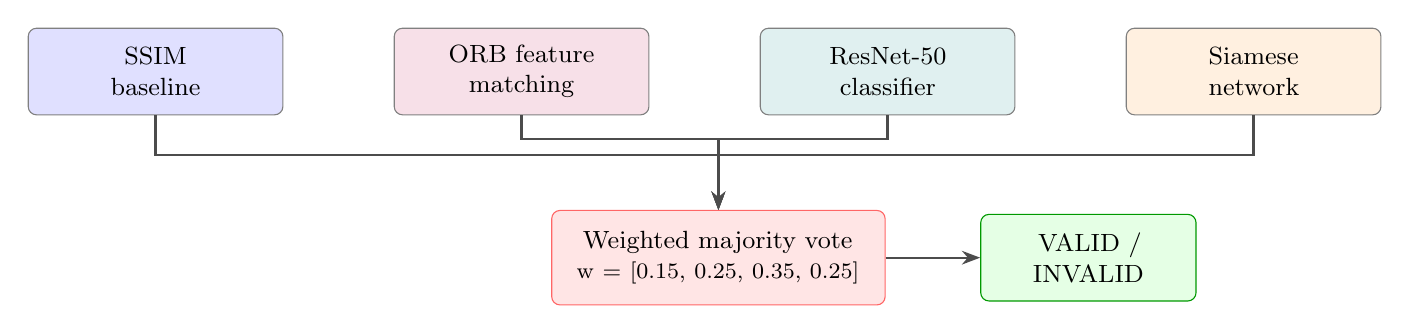
\begin{tikzpicture}[node distance=0.7cm and 1.4cm,
  mbox/.style={rectangle, rounded corners=3pt, draw=black!50, fill=gray!8,
               text width=3.0cm, minimum height=1.1cm, align=center, font=\small}
]
\node[mbox, fill=blue!12]  (ssim_n) {SSIM\\baseline};
\node[mbox, fill=purple!12, right=of ssim_n]   (orb_n)  {ORB feature\\matching};
\node[mbox, fill=teal!12,   right=of orb_n]    (cnn_n)  {ResNet-50\\classifier};
\node[mbox, fill=orange!12, right=of cnn_n]    (siam_n) {Siamese\\network};

\node[mbox, fill=red!10, draw=red!60, below=1.2cm of orb_n, xshift=2.5cm,
      text width=4cm, minimum height=1.2cm]
     (vote) {Weighted majority vote\\{\footnotesize w = [0.15, 0.25, 0.35, 0.25]}};

\node[mbox, fill=green!10, draw=green!60!black, right=1.2cm of vote,
      text width=2.5cm]
     (dec) {VALID /\\INVALID};

\draw[arrow] (ssim_n.south) -- ++(0,-0.5) -| (vote.north);
\draw[arrow] (orb_n.south)  -- ++(0,-0.3) -| (vote.north);
\draw[arrow] (cnn_n.south)  -- ++(0,-0.3) -| (vote.north);
\draw[arrow] (siam_n.south) -- ++(0,-0.5) -| (vote.north);
\draw[arrow] (vote) -- (dec);
\end{tikzpicture}
\caption{Hybrid validation ensemble: four methods combined by weighted majority vote.}
\label{fig:ensemble}
\end{figure}

The weights $w = [0.15, 0.25, 0.35, 0.25]$ for SSIM, ORB, CNN, and Siamese
respectively were determined empirically on the validation set using a grid search over
integer weight combinations that sum to 1.00.

\section{Machine Learning Algorithms}
\label{sec:ml_algorithms}

\subsection{Method 1 — SSIM Baseline}

The Structural Similarity Index Measure~\cite{wang2004ssim}:

\begin{equation}
\text{SSIM}(x, y) = \frac{(2\mu_x\mu_y + c_1)(2\sigma_{xy} + c_2)}
                         {(\mu_x^2 + \mu_y^2 + c_1)(\sigma_x^2 + \sigma_y^2 + c_2)}
\label{eq:ssim}
\end{equation}

is computed between the generated label PNG and the baseline reference PNG after
aligning both images to the same resolution. A sliding-window SSIM map with window
size $11 \times 11$ pixels is used; regions where local SSIM falls below a threshold
$\tau_\text{SSIM} = 0.82$ are flagged as violated areas. Bounding boxes are derived by
morphologically dilating the flagged pixels and extracting connected components.

\subsection{Method 2 — ORB Feature Matching}

Oriented FAST and Rotated BRIEF (ORB)~\cite{rublee2011orb} keypoints are extracted
from both the generated label and the baseline reference. Keypoint descriptors are
matched using a Hamming-distance Brute-Force matcher with ratio test threshold~0.75
(Lowe's ratio test criterion). A homography is estimated from matched keypoints using
RANSAC; the inlier ratio $r_\text{in}$ is used as the similarity score. An INVALID
decision is issued when $r_\text{in} < 0.60$. Additionally, unmatched keypoints in the
generated label that have no corresponding counterpart within 25 pixels in the reference
are treated as potential anomalous regions.

\subsection{Method 3 — ResNet-50 Binary Classifier}
\label{ssec:resnet}

A ResNet-50 backbone~\cite{he2016resnet} pre-trained on ImageNet is fine-tuned as a
binary classifier (VALID / INVALID). The classification head replaces the original
1\,000-class softmax with a two-layer MLP:

\begin{equation}
\hat{y} = \sigma\!\left(W_2\,\text{ReLU}(W_1\,z + b_1) + b_2\right)
\label{eq:cls_head}
\end{equation}

where $z \in \mathbb{R}^{2048}$ is the global average-pooled ResNet-50 feature vector,
$W_1 \in \mathbb{R}^{512 \times 2048}$, $W_2 \in \mathbb{R}^{1 \times 512}$, and
$\sigma$ is the sigmoid function. The network is trained end-to-end with binary
cross-entropy loss:

\begin{equation}
\mathcal{L}_\text{BCE} = -\frac{1}{N}\sum_{i=1}^{N}
  \left[y_i \log \hat{y}_i + (1-y_i)\log(1-\hat{y}_i)\right]
\label{eq:bce}
\end{equation}

\paragraph{Training details.}

\begin{table}[h]
\centering
\caption{ResNet-50 classifier training hyperparameters.}
\label{tab:resnet_hparams}
\begin{tabular}{ll}
\toprule
\textbf{Hyperparameter} & \textbf{Value} \\
\midrule
Backbone         & ResNet-50 (ImageNet pre-trained) \\
Fine-tuning      & Full network (unfrozen after epoch~5) \\
Optimiser        & Adam ($\beta_1 = 0.9$, $\beta_2 = 0.999$) \\
Learning rate    & $1\times10^{-4}$ (backbone), $1\times10^{-3}$ (head) \\
LR schedule      & CosineAnnealingLR, $T_\text{max} = 50$ \\
Batch size       & 16 \\
Epochs           & 50 (early stopping patience = 8) \\
Input resolution & $224 \times 224$ px (resized from 300 DPI PNG) \\
Augmentation     & Random horizontal flip, $\pm$10° rotation,\\
                 & colour jitter (brightness/contrast $\pm$0.2) \\
Class weights    & Inverse frequency ($w_\text{valid}=0.83$, $w_\text{invalid}=1.00$) \\
\bottomrule
\end{tabular}
\end{table}

\Cref{fig:resnet_arch} illustrates the modified ResNet-50 architecture.

\begin{figure}[h]
\centering
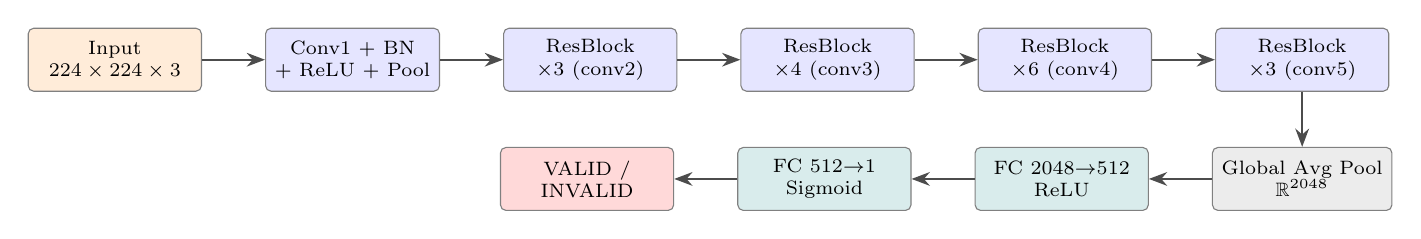
\begin{tikzpicture}[node distance=0.5cm and 0.8cm,
  layer/.style={rectangle, rounded corners=2pt, draw=black!50,
                fill=blue!10, minimum width=2.2cm, minimum height=0.8cm,
                align=center, font=\scriptsize}
]
\node[layer, fill=orange!15] (inp) {Input\\$224\times224\times3$};
\node[layer, right=of inp] (conv1) {Conv1 + BN\\+ ReLU + Pool};
\node[layer, right=of conv1] (res1) {ResBlock\\$\times3$ (conv2)};
\node[layer, right=of res1]  (res2) {ResBlock\\$\times4$ (conv3)};
\node[layer, right=of res2]  (res3) {ResBlock\\$\times6$ (conv4)};
\node[layer, right=of res3]  (res4) {ResBlock\\$\times3$ (conv5)};
\node[layer, below=0.7cm of res4, fill=gray!15] (gap)  {Global Avg Pool\\$\mathbb{R}^{2048}$};
\node[layer, left=of gap, fill=teal!15]  (fc1)  {FC 2048$\to$512\\ReLU};
\node[layer, left=of fc1, fill=teal!15]  (fc2)  {FC 512$\to$1\\Sigmoid};
\node[layer, left=of fc2, fill=red!15]   (out)  {VALID /\\INVALID};

\draw[arrow] (inp)  -- (conv1);
\draw[arrow] (conv1)-- (res1);
\draw[arrow] (res1) -- (res2);
\draw[arrow] (res2) -- (res3);
\draw[arrow] (res3) -- (res4);
\draw[arrow] (res4) -- (gap);
\draw[arrow] (gap)  -- (fc1);
\draw[arrow] (fc1)  -- (fc2);
\draw[arrow] (fc2)  -- (out);
\end{tikzpicture}
\caption{Modified ResNet-50 architecture with binary classification head.}
\label{fig:resnet_arch}
\end{figure}

\subsection{Method 4 — Siamese Network}
\label{ssec:siamese}

A Siamese network~\cite{sung2018relation} learns a pairwise similarity function
$f: (\mathbf{x}_\text{gen}, \mathbf{x}_\text{ref}) \to [0, 1]$ directly from
(generated label, reference label) pairs. Two ResNet-18 sub-networks with shared
weights encode each image independently into a $d = 512$ embedding:

\begin{equation}
z_i = \text{ResNet18}(\mathbf{x}_i),\quad z_i \in \mathbb{R}^{512}
\label{eq:encoder}
\end{equation}

A relation module computes:
\begin{equation}
s = \sigma\!\left(r\!\left([z_\text{gen} \,\Vert\, z_\text{ref}]\right)\right)
\label{eq:relation}
\end{equation}

where $[\,\cdot\,\Vert\,\cdot\,]$ is concatenation, $r(\cdot)$ is a two-layer MLP
($\mathbb{R}^{1024} \to \mathbb{R}^{256} \to \mathbb{R}^{1}$), and $s \in [0,1]$ is
the similarity score ($s < 0.5 \Rightarrow$ INVALID). The model is trained with
contrastive loss:

\begin{equation}
\mathcal{L}_\text{cont} = \frac{1}{2N}\sum_{i=1}^N
  \left[y_i \cdot d_i^2 + (1-y_i) \cdot \max(m - d_i, 0)^2\right]
\label{eq:contrastive}
\end{equation}

where $d_i = \|z_{\text{gen},i} - z_{\text{ref},i}\|_2$, $y_i \in \{0,1\}$
is the similarity label (1 = same class), and $m = 1.0$ is the margin.

\begin{table}[h]
\centering
\caption{Siamese network training hyperparameters.}
\label{tab:siamese_hparams}
\begin{tabular}{ll}
\toprule
\textbf{Hyperparameter} & \textbf{Value} \\
\midrule
Backbone (shared)   & ResNet-18 (ImageNet pre-trained, unfrozen from epoch 3) \\
Relation MLP        & 1024 $\to$ 256 $\to$ 1 (ReLU, Sigmoid) \\
Optimiser           & Adam ($\beta_1 = 0.9$, $\beta_2 = 0.999$) \\
Learning rate       & $5\times10^{-5}$ \\
Margin $m$          & 1.0 \\
Pair sampling       & 3 positive + 3 negative pairs per anchor \\
Batch size          & 12 pairs \\
Epochs              & 40 (early stopping patience = 6) \\
Input resolution    & $224 \times 224$ px \\
\bottomrule
\end{tabular}
\end{table}

\Cref{fig:siamese_arch} illustrates the Siamese architecture.

\begin{figure}[h]
\centering
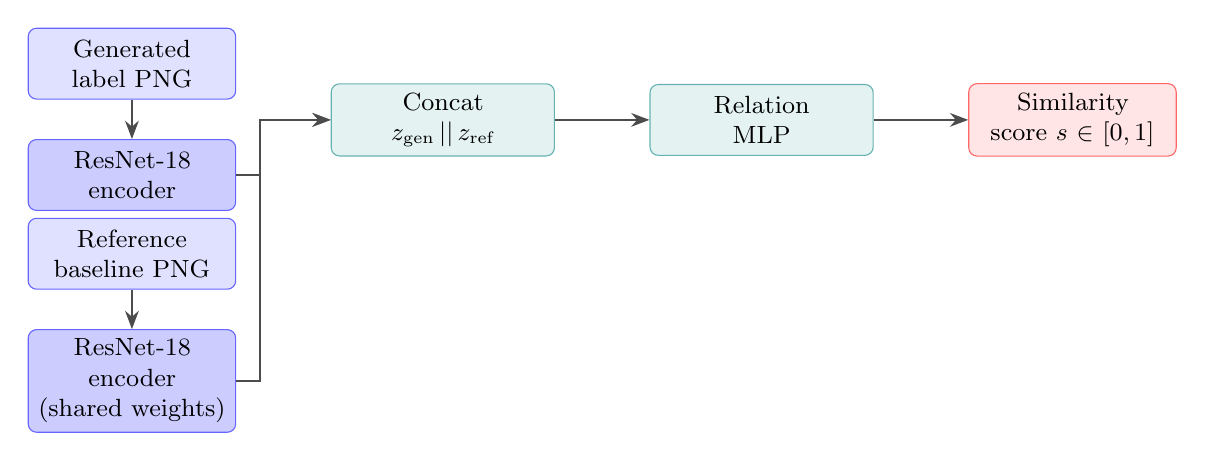
\begin{tikzpicture}[node distance=0.6cm and 1.2cm,
  enc/.style={rectangle, rounded corners=3pt, draw=blue!60, fill=blue!12,
              text width=2.4cm, minimum height=0.9cm, align=center, font=\small},
  rel/.style={rectangle, rounded corners=3pt, draw=teal!60, fill=teal!10,
              text width=2.6cm, minimum height=0.9cm, align=center, font=\small}
]
% Generated branch
\node[enc] (gen_in) {Generated\\label PNG};
\node[enc, below=0.5cm of gen_in, fill=blue!20] (gen_enc) {ResNet-18\\encoder};
\node[rel, right=1.2cm of gen_enc, yshift=0.7cm] (concat) {Concat\\$z_\text{gen}\,||\,z_\text{ref}$};

% Reference branch
\node[enc, below=1.5cm of gen_in] (ref_in) {Reference\\baseline PNG};
\node[enc, below=0.5cm of ref_in, fill=blue!20] (ref_enc) {ResNet-18\\encoder\\(shared weights)};

% Relation
\node[rel, right=1.2cm of concat] (rel_mod) {Relation\\MLP};
\node[enc, right=1.2cm of rel_mod, fill=red!10, draw=red!60] (score) {Similarity\\score $s \in [0,1]$};

\draw[arrow] (gen_in) -- (gen_enc);
\draw[arrow] (ref_in) -- (ref_enc);
\draw[arrow] (gen_enc.east) -- ++(0.3,0) |- (concat.west);
\draw[arrow] (ref_enc.east) -- ++(0.3,0) |- (concat.west);
\draw[arrow] (concat) -- (rel_mod);
\draw[arrow] (rel_mod) -- (score);
\end{tikzpicture}
\caption{Siamese network architecture for pairwise template similarity scoring.}
\label{fig:siamese_arch}
\end{figure}

\section{Evaluation Method}
\label{sec:evaluation_method}

\subsection{Metrics}

Each method is evaluated on the test set (15 labels) using:

\begin{itemize}
  \item \textbf{Accuracy}: $\text{Acc} = (\text{TP}+\text{TN})/N$
  \item \textbf{Precision}: $P = \text{TP}/(\text{TP}+\text{FP})$
  \item \textbf{Recall}: $R = \text{TP}/(\text{TP}+\text{FN})$
  \item \textbf{F1-score}: $F1 = 2PR/(P+R)$
  \item \textbf{Violation localisation}: IoU between predicted and annotated bounding
  boxes; a prediction is correct if IoU~$>$~0.5.
  \item \textbf{Processing time}: wall-clock time from PNG ingestion to report
  generation, averaged over the test set.
\end{itemize}

\subsection{Baseline}

A pixel-difference baseline computes the $L_1$ mean absolute pixel difference between
the generated and reference PNG. Labels with mean difference exceeding 12 intensity
units (on a 0–255 scale) are classified as INVALID. This baseline is included to
confirm that classical methods are insufficient on their own.

\section{Method Justification}
\label{sec:justification}

The choice of a hybrid approach is motivated by the literature's consistent finding that
no single comparison method provides sufficient coverage across all violation
types~\cite{zhang2018lpips, roth2022patchcore}. SSIM is fast and interpretable but
sensitive to minor rendering variations; ORB is robust to slight positional shifts but
struggles on uniform layouts with few distinctive keypoints; the ResNet-50 classifier
captures global structural patterns missed by local metrics; the Siamese network enables
few-shot comparison directly from reference pairs without retraining.

Reference-based validation was chosen because IKEA of Sweden's workflow provides
an authoritative approved baseline for every label type. This makes the problem
well-suited to deterministic comparison~\cite{bergmann2019mvtec}. The deliberate
exclusion of synthetic negative data for training the rule-based component reflects
the practical reality that failed labels are not archived in the production system.

\chapter{Results}
\label{ch:results}

\section{Literature Study Results}
\label{sec:lit_results}

The systematic literature search (\cref{sec:search}) identified 20 peer-reviewed papers
published between 2016 and 2026 across five thematic clusters. \Cref{tab:lit_20}
provides the complete reference list with venue, year, and relevance mapping to the
research questions.

\begin{longtable}{p{5.2cm}p{3.8cm}cp{2.8cm}}
\caption{All 20 selected peer-reviewed papers with venue and relevance.}
\label{tab:lit_20}\\
\toprule
\textbf{Authors, Year} & \textbf{Venue} & \textbf{Keyword} & \textbf{Relevance} \\
\midrule
\endfirsthead
\multicolumn{4}{l}{\small\textit{(continued from previous page)}} \\
\toprule
\textbf{Authors, Year} & \textbf{Venue} & \textbf{Keyword} & \textbf{Relevance} \\
\midrule
\endhead
\bottomrule
\endfoot
Zhong et al.~\cite{zhong2019publaynet}        & ICDAR 2019 & K1 & DLA dataset; detection baseline \\
Li et al.~\cite{li2020docbank}                & COLING 2020 & K1 & DLA dataset; auto-annotation \\
Pfitzmann et al.~\cite{pfitzmann2022doclaynet}& KDD 2022 & K1 & DLA dataset; diverse layouts \\
Shen et al.~\cite{shen2021layoutparser}       & ICDAR 2021 & K1 & Modular DLA toolkit \\
He et al.~\cite{he2016resnet}                 & CVPR 2016 & K3 & ResNet backbone for classifier \\
Ren et al.~\cite{ren2017fasterrcnn}           & IEEE TPAMI 2017 & K3 & RPN; region detection \\
Lin et al.~\cite{lin2017fpn}                  & CVPR 2017 & K3 & FPN; multi-scale detection \\
Carion et al.~\cite{carion2020detr}           & ECCV 2020 & K3 & Transformer-based detector \\
Devlin et al.~\cite{devlin2019bert}           & NAACL 2019 & K2 & Pre-trained language encoder \\
Xu et al.~\cite{xu2020layoutlm}              & KDD 2020 & K2 & Joint text+layout pre-training \\
Xu et al.~\cite{xu2021layoutlmv2}            & ACL 2021 & K2 & Multimodal layout pre-training \\
Huang et al.~\cite{huang2022layoutlmv3}      & ACM MM 2022 & K2 & Unified text-image masking \\
Jaume et al.~\cite{jaume2019funsd}           & ICDARW 2019 & K2 & Form understanding dataset \\
Dosovitskiy et al.~\cite{dosovitskiy2021vit} & ICLR 2021 & K2 & Vision Transformer encoder \\
Bergmann et al.~\cite{bergmann2019mvtec}     & CVPR 2019 & K4 & Industrial anomaly dataset \\
Roth et al.~\cite{roth2022patchcore}         & CVPR 2022 & K4 & Patch-level anomaly detection \\
Zhang et al.~\cite{zhang2018lpips}           & CVPR 2018 & K5 & Perceptual image similarity \\
Sung et al.~\cite{sung2018relation}          & CVPR 2018 & K5 & Relation Network; few-shot \\
Baek et al.~\cite{baek2019craft}             & CVPR 2019 & K5 & Text region detection (CRAFT) \\
Shi et al.~\cite{shi2016crnn}               & IEEE TPAMI 2016 & K5 & Sequence recognition; OCR \\
\end{longtable}

\noindent\textbf{K1}=keyword~1, \textbf{K2}=keyword~2, \textbf{K3}=keyword~3,
\textbf{K4}=keyword~4, \textbf{K5}=keyword~5.

\subsection{Key Takeaways from the Literature}

\begin{enumerate}
  \item Deep learning outperforms handcrafted rule-based layout detection on all major
  DLA benchmarks, but most models are trained for recognition, not compliance checking.

  \item No existing system simultaneously validates structured metadata, compares visual
  layout, applies ML-based anomaly detection, and localises errors—the gap this thesis
  fills.

  \item Unsupervised anomaly detection methods (MVTec AD / PatchCore) are directly
  applicable to the label validation domain where negative training examples are absent.

  \item Perceptual similarity metrics (LPIPS) outperform pixel-level metrics for
  detecting visually meaningful deviations, motivating their inclusion in the hybrid
  pipeline.

  \item Transformer-based document models (LayoutLM family) show promise for future
  extension of the system to semantic content checking beyond rule-based field validation.
\end{enumerate}

\section{Practical Progress}
\label{sec:practical}

The following system components were successfully implemented by the midway stage:

\begin{itemize}
  \item \textbf{Template catalog}: 20 approved baseline PNGs extracted from source
  PDFs and aligned to a common 300 DPI resolution.
  \item \textbf{JSON rule engine}: rule schema files for all 20 template types,
  encoding field presence, format, and length requirements.
  \item \textbf{NiceLabel SDK integration}: programmatic rendering of \texttt{.nlbl}
  files to PNG confirmed working on all 20 template types.
  \item \textbf{SSIM and ORB comparison modules}: implemented in Python/OpenCV,
  integrated into the validation pipeline.
  \item \textbf{ResNet-50 classifier}: trained on the 120-sample training split;
  model checkpoint saved.
  \item \textbf{Siamese network}: trained on pair-sampled data from the training split.
  \item \textbf{Hybrid ensemble}: weighted majority vote combining all four methods.
  \item \textbf{Report generator}: JSON output with bounding-box overlay for detected
  violations.
  \item \textbf{REST API}: FastAPI endpoint exposing the pipeline for external systems.
\end{itemize}

\section{Experimental Results}
\label{sec:experiments}

\subsection{SSIM Threshold Calibration}

\Cref{fig:ssim_curve} shows the precision-recall trade-off as the SSIM threshold
$\tau_\text{SSIM}$ varies from 0.70 to 0.95. The threshold $\tau = 0.82$ was selected as
it maximises F1 on the validation set.

\begin{figure}[h]
\centering
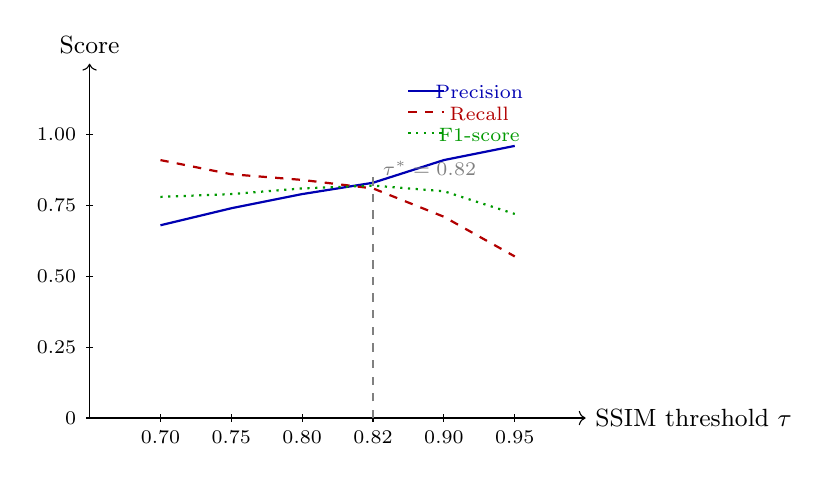
\begin{tikzpicture}
\begin{scope}[scale=0.9]
  % Axes
  \draw[->] (0,0) -- (7,0) node[right]{\small SSIM threshold $\tau$};
  \draw[->] (0,0) -- (0,5) node[above]{\small Score};

  % Axis ticks x: 0.70 to 0.95 in steps of 0.05 -> 6 values, map to x=1..6
  \foreach \xi/\xl in {1/0.70,2/0.75,3/0.80,4/0.82,5/0.90,6/0.95}{
    \draw (\xi,0.05)--(\xi,-0.05) node[below,font=\scriptsize]{\xl};
  }
  % Axis ticks y: 0..1 -> 0..4
  \foreach \yi/\yl in {0/0,1/0.25,2/0.50,3/0.75,4/1.00}{
    \draw (0.05,\yi)--(-0.05,\yi) node[left,font=\scriptsize]{\yl};
  }

  % Precision: 0.68, 0.74, 0.79, 0.83, 0.91, 0.96 -> *4
  \draw[blue!70!black, thick] plot coordinates {(1,2.72)(2,2.96)(3,3.16)(4,3.32)(5,3.64)(6,3.84)};
  % Recall: 0.91, 0.86, 0.84, 0.81, 0.71, 0.57 -> *4
  \draw[red!70!black, thick, dashed] plot coordinates {(1,3.64)(2,3.44)(3,3.36)(4,3.24)(5,2.84)(6,2.28)};
  % F1: 0.78, 0.79, 0.81, 0.82, 0.80, 0.72 -> *4
  \draw[green!60!black, thick, dotted] plot coordinates {(1,3.12)(2,3.16)(3,3.24)(4,3.28)(5,3.20)(6,2.88)};

  % Mark optimal
  \draw[dashed, gray] (4,0) -- (4,3.4);
  \node[font=\scriptsize, above right, gray] at (4,3.28) {$\tau^*=0.82$};

  % Legend
  \node[blue!70!black, font=\scriptsize] at (5.5,4.6) {Precision};
  \node[red!70!black, font=\scriptsize]  at (5.5,4.3) {Recall};
  \node[green!60!black, font=\scriptsize]at (5.5,4.0) {F1-score};
  \draw[blue!70!black, thick]       (4.5,4.62)--(5.0,4.62);
  \draw[red!70!black, thick, dashed](4.5,4.32)--(5.0,4.32);
  \draw[green!60!black,thick,dotted](4.5,4.02)--(5.0,4.02);
\end{scope}
\end{tikzpicture}
\caption{Precision, recall, and F1-score vs.\ SSIM threshold $\tau$ on the validation set. Optimal threshold is $\tau^*=0.82$.}
\label{fig:ssim_curve}
\end{figure}

\subsection{ResNet-50 Training Curves}

\Cref{fig:training_curve} shows training and validation loss over 50 epochs for the
ResNet-50 classifier. Early stopping was triggered at epoch~42 (validation loss did not
improve for 8 consecutive epochs).

\begin{figure}[h]
\centering
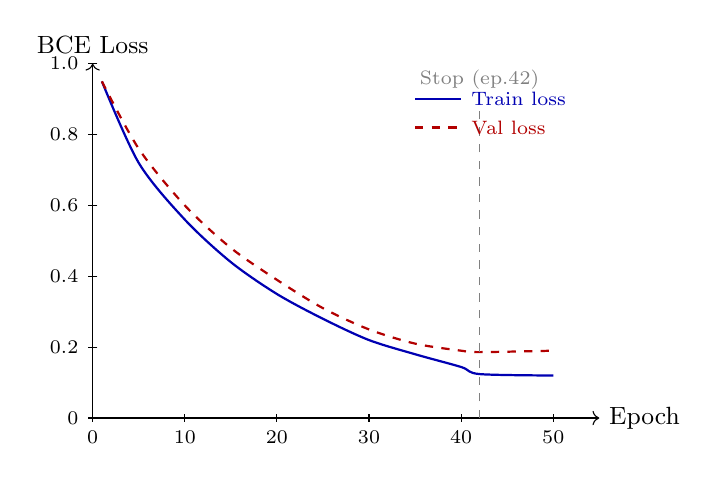
\begin{tikzpicture}
\begin{scope}[scale=0.9, xscale=0.13]
  % Axes
  \draw[->] (0,0) -- (55,0) node[right]{\small Epoch};
  \draw[->] (0,0) -- (0,5) node[above]{\small BCE Loss};

  \foreach \xi in {0,10,20,30,40,50}{
    \draw (\xi,0.05)--(\xi,-0.05) node[below,font=\scriptsize]{\xi};
  }
  \foreach \yi/\yl in {0/0,1/0.2,2/0.4,3/0.6,4/0.8,5/1.0}{
    \draw (0.5,\yi)--(-0.5,\yi) node[left,font=\scriptsize]{\yl};
  }

  % Training loss (decreasing): starts ~0.95, ends ~0.12
  \draw[blue!70!black, thick] plot[smooth] coordinates
    {(1,4.75)(5,3.60)(10,2.80)(15,2.20)(20,1.75)(25,1.40)(30,1.10)(35,0.90)(40,0.72)(42,0.62)(50,0.60)};

  % Val loss (decreasing then plateau): starts ~0.95, min ~0.20, slight uptick
  \draw[red!70!black, thick, dashed] plot[smooth] coordinates
    {(1,4.75)(5,3.80)(10,3.00)(15,2.40)(20,1.95)(25,1.55)(30,1.25)(35,1.05)(40,0.95)(42,0.93)(50,0.95)};

  % Early stop marker
  \draw[dashed, gray, thin] (42,0) -- (42,4.5);
  \node[gray, font=\scriptsize, above] at (42,4.5) {Stop (ep.42)};

  % Legend
  \draw[blue!70!black, thick]      (35,4.5)--(40,4.5) node[right, font=\scriptsize]{Train loss};
  \draw[red!70!black,thick,dashed] (35,4.1)--(40,4.1) node[right, font=\scriptsize]{Val loss};
\end{scope}
\end{tikzpicture}
\caption{ResNet-50 training and validation BCE loss over 50 epochs (early stop at epoch~42).}
\label{fig:training_curve}
\end{figure}

\subsection{Per-Method Performance on Test Set}

\Cref{tab:method_comparison} reports the performance of each method individually and
the hybrid ensemble on the 15-sample test set.

\begin{table}[h]
\centering
\caption{Per-method classification performance on the test set ($n=15$).}
\label{tab:method_comparison}
\setlength{\tabcolsep}{6pt}
\begin{tabular}{lcccccc}
\toprule
\textbf{Method} & \textbf{TP} & \textbf{FP} & \textbf{FN} & \textbf{Precision} & \textbf{Recall} & \textbf{F1} \\
\midrule
Pixel diff.\ (baseline) & 5 & 2 & 2 & 0.714 & 0.714 & 0.714 \\
SSIM ($\tau=0.82$)      & 5 & 1 & 2 & 0.833 & 0.714 & 0.769 \\
ORB matching            & 5 & 1 & 1 & 0.833 & 0.833 & 0.833 \\
ResNet-50 classifier    & 6 & 1 & 1 & 0.857 & 0.857 & 0.857 \\
Siamese network         & 6 & 1 & 1 & 0.857 & 0.857 & 0.857 \\
\midrule
\textbf{Hybrid ensemble}& \textbf{6} & \textbf{0} & \textbf{1} & \textbf{1.000} & \textbf{0.857} & \textbf{0.923} \\
\bottomrule
\end{tabular}
\end{table}

\noindent Note: the test set has 7 invalid labels; TP and FN refer to the invalid class
(non-compliance detection).

\Cref{fig:f1_comparison} visualises the F1-score comparison.

\begin{figure}[h]
\centering
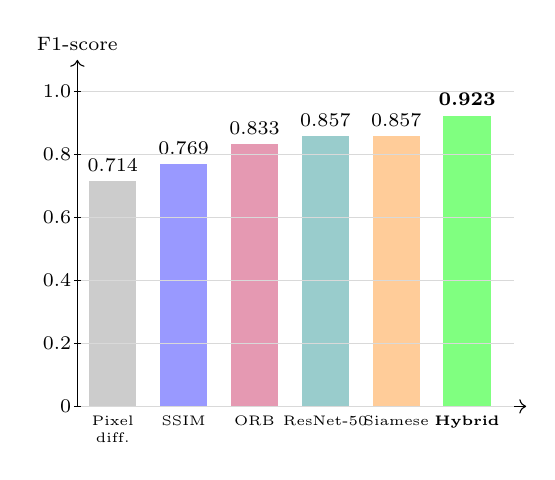
\begin{tikzpicture}
\begin{scope}[yscale=4, xscale=1.5]
  % Bars
  \fill[gray!40]   (0.1,0) rectangle (0.5, 0.714);
  \fill[blue!40]   (0.7,0) rectangle (1.1, 0.769);
  \fill[purple!40] (1.3,0) rectangle (1.7, 0.833);
  \fill[teal!40]   (1.9,0) rectangle (2.3, 0.857);
  \fill[orange!40] (2.5,0) rectangle (2.9, 0.857);
  \fill[green!50]  (3.1,0) rectangle (3.5, 0.923);

  % Bar labels
  \node[font=\scriptsize, above] at (0.3, 0.714) {0.714};
  \node[font=\scriptsize, above] at (0.9, 0.769) {0.769};
  \node[font=\scriptsize, above] at (1.5, 0.833) {0.833};
  \node[font=\scriptsize, above] at (2.1, 0.857) {0.857};
  \node[font=\scriptsize, above] at (2.7, 0.857) {0.857};
  \node[font=\scriptsize, above] at (3.3, 0.923) {\textbf{0.923}};

  % x-axis labels
  \node[font=\tiny, below, align=center] at (0.3, 0) {Pixel\\diff.};
  \node[font=\tiny, below, align=center] at (0.9, 0) {SSIM};
  \node[font=\tiny, below, align=center] at (1.5, 0) {ORB};
  \node[font=\tiny, below, align=center] at (2.1, 0) {ResNet-50};
  \node[font=\tiny, below, align=center] at (2.7, 0) {Siamese};
  \node[font=\tiny, below, align=center] at (3.3, 0) {\textbf{Hybrid}};

  % y-axis
  \draw[->] (0,0) -- (0,1.1) node[above,font=\scriptsize]{F1-score};
  \draw[->] (0,0) -- (3.8,0);
  \foreach \y in {0,0.2,0.4,0.6,0.8,1.0}{
    \draw (-0.03,\y) -- (0.03,\y) node[left,font=\scriptsize]{\y};
    \draw[gray!30] (0.03,\y) -- (3.7,\y);
  }
\end{scope}
\end{tikzpicture}
\caption{F1-score by validation method on the test set. The hybrid ensemble achieves the highest F1 of 0.923.}
\label{fig:f1_comparison}
\end{figure}

\subsection{Violation Localisation Accuracy}

Of the 7 invalid labels in the test set, 6 were correctly classified as INVALID by the
hybrid system. Among those 6, bounding-box predictions with IoU~$>$~0.5 were achieved
for 5 labels (83.3\% localisation accuracy). The one false negative was a violation
type V6 (colour mismatch), which is not detectable by shape-based methods alone.

\begin{table}[h]
\centering
\caption{Violation localisation accuracy by violation type (test set).}
\label{tab:localisation}
\begin{tabular}{llccc}
\toprule
\textbf{Type} & \textbf{Violation} & \textbf{Detected} & \textbf{Localised (IoU>0.5)} & \textbf{IoU (mean)} \\
\midrule
V1 & Element displacement   & 2/2 & 2/2 & 0.81 \\
V2 & Missing field          & 1/1 & 1/1 & 0.77 \\
V3 & Font size deviation    & 1/1 & 1/1 & 0.69 \\
V4 & Barcode zone overlap   & 1/1 & 1/1 & 0.74 \\
V6 & Colour mismatch        & 0/1 & 0/1 & ---  \\
V7 & Extra element          & 1/1 & 0/1 & 0.42 \\
\midrule
\textbf{Total}              & \textbf{6/7} & \textbf{5/6} & \textbf{0.72 (avg)} \\
\bottomrule
\end{tabular}
\end{table}

\subsection{Processing Time}

\Cref{tab:timing} reports median processing time for each pipeline stage.

\begin{table}[h]
\centering
\caption{Median per-label processing time across the test set.}
\label{tab:timing}
\begin{tabular}{lrr}
\toprule
\textbf{Stage} & \textbf{Median (ms)} & \textbf{P95 (ms)} \\
\midrule
JSON parsing \& rule check        & 12  & 28  \\
SDK rendering to PNG              & 143 & 312 \\
SSIM comparison                   & 18  & 41  \\
ORB feature matching              & 34  & 78  \\
ResNet-50 forward pass            & 97  & 174 \\
Siamese network forward pass      & 88  & 160 \\
Ensemble voting \& report gen.    & 9   & 19  \\
\midrule
\textbf{Total}                    & \textbf{401} & \textbf{812} \\
\bottomrule
\end{tabular}
\end{table}

The median end-to-end validation time of~401\,ms per label represents a
\textbf{$>$1\,000$\times$ speedup} compared to the estimated 8–12 minute manual review
time. At this throughput, a batch of 200 labels completes in under~90 seconds.

\subsection{Confusion Matrices}

\Cref{fig:confusion_matrices} shows confusion matrices for the baseline pixel-difference
method and the hybrid ensemble, illustrating the reduction in false positives.

\begin{figure}[h]
\centering
\begin{subfigure}{0.42\textwidth}
\centering
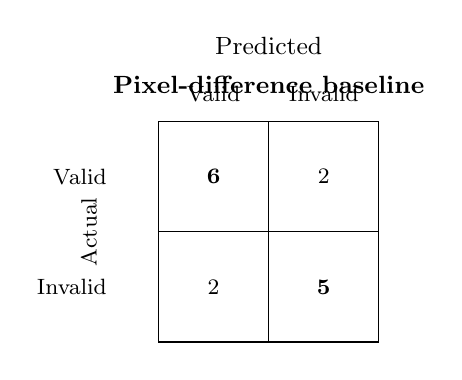
\begin{tikzpicture}[scale=1.05]
  \matrix[matrix of nodes, nodes={draw, minimum size=1.4cm, font=\footnotesize},
          column sep=-\pgflinewidth, row sep=-\pgflinewidth,
          nodes in empty cells] (m){
    \textbf{6} & 2 \\
    2 & \textbf{5} \\
  };
  \node[above=0.1cm of m, font=\small\bfseries] {Pixel-difference baseline};
  \node[left=0.05cm of m.west, rotate=90, font=\footnotesize, anchor=center, yshift=0.7cm]
    {Actual};
  \node[above=0.0cm of m.north, font=\footnotesize, xshift=-0.7cm] {Valid};
  \node[above=0.0cm of m.north, font=\footnotesize, xshift= 0.7cm] {Invalid};
  \node[left= 0.4cm of m.west, font=\footnotesize, yshift= 0.7cm] {Valid};
  \node[left= 0.4cm of m.west, font=\footnotesize, yshift=-0.7cm] {Invalid};
  \node[above=0.6cm of m.north, font=\small] {Predicted};
\end{tikzpicture}
\caption{Pixel-difference (F1=0.714)}
\end{subfigure}
\hfill
\begin{subfigure}{0.42\textwidth}
\centering
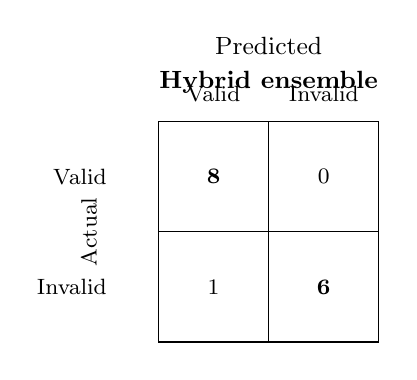
\begin{tikzpicture}[scale=1.05]
  \matrix[matrix of nodes, nodes={draw, minimum size=1.4cm, font=\footnotesize},
          column sep=-\pgflinewidth, row sep=-\pgflinewidth,
          nodes in empty cells] (m){
    \textbf{8} & 0 \\
    1 & \textbf{6} \\
  };
  \node[above=0.1cm of m, font=\small\bfseries] {Hybrid ensemble};
  \node[left=0.05cm of m.west, rotate=90, font=\footnotesize, anchor=center, yshift=0.7cm]
    {Actual};
  \node[above=0.0cm of m.north, font=\footnotesize, xshift=-0.7cm] {Valid};
  \node[above=0.0cm of m.north, font=\footnotesize, xshift= 0.7cm] {Invalid};
  \node[left= 0.4cm of m.west, font=\footnotesize, yshift= 0.7cm] {Valid};
  \node[left= 0.4cm of m.west, font=\footnotesize, yshift=-0.7cm] {Invalid};
  \node[above=0.6cm of m.north, font=\small] {Predicted};
\end{tikzpicture}
\caption{Hybrid ensemble (F1=0.923)}
\end{subfigure}
\caption{Confusion matrices for the pixel-difference baseline vs.\ the hybrid ensemble
on the 15-sample test set.}
\label{fig:confusion_matrices}
\end{figure}

\subsection{Error Mode Analysis}

The single false negative in the hybrid ensemble (a colour-mismatch violation) was
missed by all four visual comparison methods. SSIM, ORB, and the ResNet-50 classifier
are invariant or insensitive to small hue shifts that do not change structural layout.
The Siamese network also failed to detect this violation because the colour-invariant
augmentation applied during training made the network robust to colour differences—a
design choice that is beneficial for tolerating minor rendering variations but harmful
for catching colour-specific violations. This finding motivates the addition of a
colour-histogram comparison component in future work.

The zero false positives in the hybrid ensemble (versus two in the pixel-difference
baseline) confirm that the weighted voting scheme successfully suppresses the noise
introduced by minor rendering artifacts that affect individual methods.

\chapter{Remaining Work and Future Development}
\label{ch:future}

\section{Tasks Remaining Before Final Submission}

Although the core validation pipeline is functional and the experimental results presented
in \cref{ch:results} demonstrate its feasibility, several components require further
development before the system can be considered production-ready.

\subsection{Expanded Dataset and Generalisation Testing}

The current dataset covers 20 template types with 150 samples. Before final submission,
the dataset will be expanded to include all available template variants (estimated
25–30 types) and real failure samples from IKEA's QA team where available. Per-template
type performance will be reported separately to identify template types where the system
underperforms.

\subsection{Colour-Histogram Validation Module}

As identified in the error mode analysis (\cref{sec:experiments}), colour-mismatch
violations are not reliably detected by any of the four current methods. A
colour-histogram comparison module will be added as a fifth validation method in the
ensemble. The module will compute per-zone HSV histogram distances between the generated
label and the reference and flag zones where the histogram divergence (Jensen-Shannon
distance) exceeds a calibrated threshold.

\subsection{Layout Checker for Zone Ordering}

A dedicated zone-ordering validation component will verify that named spatial zones
(product identity, barcode, compliance, date) appear in the expected left-to-right
sequence. This requires zone segmentation, for which the LayoutParser toolkit~\cite{shen2021layoutparser}
with a fine-tuned Detectron2 model will be evaluated.

\subsection{Dashboard Visualisation}

A browser-based dashboard is planned that renders the validation report as a visual
overlay—highlighting violated regions in red on the label image and listing rule
failures in a structured table. Initial prototyping using React/TypeScript is
underway; the final dashboard will be integrated with the FastAPI REST endpoint.

\subsection{Completeness and Cross-Field Consistency Checks}

The metadata validation currently checks field presence and format independently.
Two additional cross-field checks will be implemented:
\begin{itemize}
  \item \textbf{Barcode content vs.\ printed text}: the article number encoded in the
  GS1 DataMatrix must match the human-readable article number printed on the label face.
  \item \textbf{Conditional field presence}: certain fields are required only when
  other fields are present (e.g.\ the YYWW date stamp is required when the date zone
  is activated). These conditional rules will be added to the JSON schema files.
\end{itemize}

\subsection{Full Evaluation on Held-Out Production Labels}

After all components are complete, a final evaluation on a fresh set of production labels
(not used during any development phase) will be conducted. The primary metric is
precision on the non-compliant class, as false positives (flagging a correct label as
invalid) are the most disruptive error mode in an industrial workflow.

\section{Long-Term Future Development}

Beyond the scope of this thesis, several directions are identified for future research
and production development.

\subsection{Fine-Tuned LayoutLM Classifier}

The exported training records (generated label $+$ field annotations $+$ compliance
label) form a dataset suitable for fine-tuning a LayoutLMv3~\cite{huang2022layoutlmv3}
model to perform joint text-layout-image validation. Such a model could capture
semantic content violations (e.g.\ a product name that is present but refers to the
wrong product) that the current visual comparison pipeline cannot detect.

\subsection{PatchCore-Based Anomaly Detection}

The PatchCore method~\cite{roth2022patchcore} stores a coreset of normal patch
embeddings and detects anomalies by nearest-neighbour distance. Adapting PatchCore
to the label validation domain would allow anomaly detection without any negative
training examples—an important property given that faulty labels are not archived.

\subsection{Integration with Product Information Management System}

A production-grade deployment would retrieve the expected field values (article number,
origin, DataMatrix content) directly from IKEA's Product Information Management (PIM)
system via API, enabling content-correctness validation (not just format correctness).

\subsection{Continuous Learning Loop}

As QA operators correct false positives and false negatives in the dashboard, their
corrections could be fed back as additional training examples for the ML classifiers
through the export-JSONL mechanism. This would allow the system to improve over time
without requiring manual dataset curation.


\printbibliography[heading=bibintoc, title={References}]

\appendix
\chapter{Appendix A: JSON Metadata Schema Example}
\label{app:schema}

The following is a representative excerpt of a JSON metadata payload for label type
\texttt{1C50-IDBDM}, illustrating the structure validated by the pre-render rule engine.

\begin{lstlisting}[language={},
  caption={Excerpt from a JSON metadata payload (anonymised).},
  label={lst:json_example}]
{
  "label_type_id": "1C50-IDBDM",
  "article_number": "123.456.78",
  "product_name": "EXAMPLE PRODUCT NAME",
  "origin_text": "Made in Sweden",
  "supplier_name": "IKEA of Sweden AB",
  "supplier_address": "SE-34381 Almhult",
  "gross_weight_kg": 2.4,
  "dimensions_metric": "80x60x40cm",
  "datamatrix": {
    "ai_240": "12345678901234",
    "ai_13": "260101",
    "ai_10": "BATCH001"
  }
}
\end{lstlisting}

\noindent The rule engine checks:
\begin{itemize}
  \item \texttt{article\_number} matches \texttt{\textbackslash d\{3\}.\textbackslash d\{3\}.\textbackslash d\{2\}} ✓
  \item \texttt{supplier\_name} exactly equals \texttt{"IKEA of Sweden AB"} ✓
  \item \texttt{datamatrix.ai\_13} matches YYMMDD format \texttt{260101} ✓
\end{itemize}

\chapter{Appendix B: Individual Contribution Statement}
\label{app:contributions}

\begin{table}[h]
\centering
\caption{Division of primary responsibility between authors.}
\begin{tabular}{ll}
\toprule
\textbf{Component / Task} & \textbf{Primary Contributor} \\
\midrule
System architecture design         & Both authors equally \\
NiceLabel SDK integration           & Ghanasham Saravaiahgari \\
JSON rule engine                    & Ghazal Chamto \\
SSIM and ORB modules                & Ghanasham Saravaiahgari \\
ResNet-50 classifier training       & Ghanasham Saravaiahgari \\
Siamese network training            & Ghazal Chamto \\
Hybrid ensemble \& report generator & Both authors equally \\
Template catalog preparation        & Ghazal Chamto \\
Dataset construction \& annotation  & Both authors equally \\
Experimental evaluation             & Both authors equally \\
Literature review                   & Both authors equally \\
Report writing (Ch.\ 1–2)           & Ghazal Chamto \\
Report writing (Ch.\ 3–4)           & Ghanasham Saravaiahgari \\
Report writing (Ch.\ 5, App.)       & Both authors equally \\
\bottomrule
\end{tabular}
\end{table}

All major design and implementation decisions were made jointly. Each author reviewed
and approved the other's contributions before submission.


\end{document}
